\section{Proposta}
\label{sec:proposta}

\subsection{A aplicação Price Search}

A aplicação Price Search foi pensada com o intuito de facilitar a pesquisa de preço de quaisquer tipos de itens existentes no mercado, sejam eles eletrodomésticos, alimentos, utensílios, remédios, etc. Hoje em dia é possível ncontrar diversos tipos de produtos em \textit{sites} de grandes lojas, porém, como há várias cidades no Brasil que não são atendidas por tais estabelecimentos, percebe-se que há uma grande dificuldade para determinar qual lugar oferece tal produto com o menor custo. Com isso, a ideia da aplicação é que as pessoas tenham acesso a um recurso para comparação de preço dos produtos dos estabelecimentos locais, a fim de ajudar as pessoas a economizar dinheiro. 

Outra finalidade da aplicação é ajudar na busca de produtos, dos quais anteriormente não se sabia onde eram vendidos. Com uma simples pesquisa, o usuário pode identificar facilmente o valor desses produtos e onde encontrá-los, por meio de um mapa que fornece a localização do estabelecimento contendo o seu endereço. 

O intuito é criar uma ferramenta simples, de fácil uso e multiplataforma, com o objetivo de agregar a quantidade máxima de usuários possíveis, para que todos possam usá-la de maneira rápida e eficiente.

\subsection{CRUD}
No projeto há \textit{CRUDs} (do inglês, \textit{Create, Read, Update \& Delete}) que irão realizar operações básicas como criação, recuperação, atualização ou remoção das informações persistidas no banco de dados, como produtos, listas de compras, ofertas, estabelecimentos e usuários. 

\subsection{Progressive Web App}

O \textit{PWA} é uma metodologia de desenvolvimento de aplicações \textit{web} que também se comportem como aplicações nativas, de modo que sua concepção seja facilitada. Ela utiliza \textit{service workers}, que são \textit{scripts} que fazem o gerenciamento do \textit{cache}\footnote{Memória temporária comumente utilizada para armazenar recursos frequentemente acessados por processos.}, fornecendo um melhor desempenho pois os dados e boa parte do \textit{front-end} são persistidos no próprio dispositivo.

Mesmo sendo uma aplicação \textit{web}, o \textit{PWA} pode acessar diversos recursos do dispositivo, como o \textit{GPS} (do inglês, \textit{Global Positioning System}), podendo portanto, ser usada de forma dinâmica.

Diferentemente dos aplicativos que devem ser baixados de uma loja, a única coisa que o usuário precisa fazer é entrar no \textit{site} da aplicação \textit{web} e, caso tenha interesse, pode salva-la em seu dispositivo, como se fosse uma aplicação móvel. Inclusive, o Google Play Store\footnote{Loja de aplicativos voltada para dispositivos móveis Android. Disponível em \url{https://play.google.com/store}.} também se abriu para aplicações \textit{PWA}, tornando sua distribuição retrocompatível com o método convencional.

A aplicação foi desenvolvida em PWA por ser uma tecnologia em ascensão, que permite desenvolver utilizando tecnologias \textit{web} e funciona com se fosse uma aplicação nativa, seja no \textit{smartphone} ou no computador. O PWA hoje conta com forte apoio de empresas gigantes da \textit{web}, como o Google, Microsoft e Mozilla, e alguns exemplos de grande sucesso no mercado são o Tinder, AliExpress, Pinterest, entre outros.

\subsection{Diagrama de Blocos}

 O diagrama de blocos (ilustrado na Figura  \ref{fig:diagrama_de_blocos}) é uma representação gráfica de todas as tecnologias que foram utilizadas no desenvolvimento do projeto, bem como sobre como é feita a comunicação entre elas.
 
\begin{figure}[!htb]
\centering
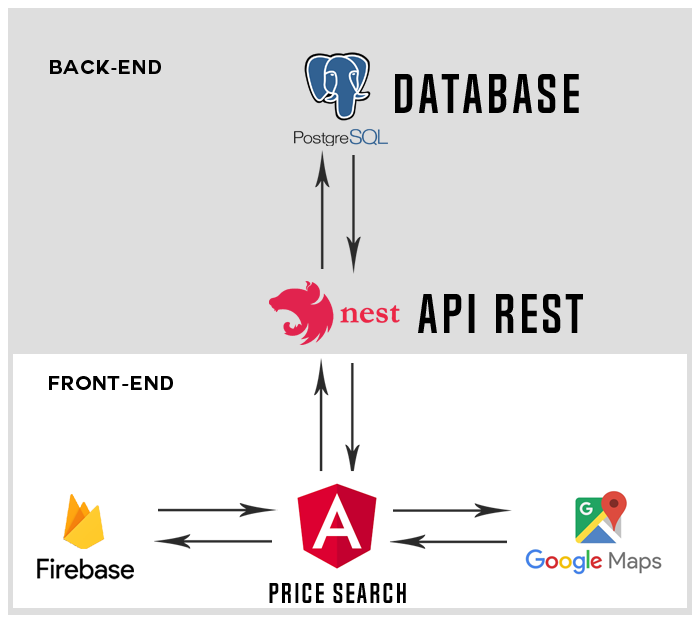
\includegraphics[width=\linewidth]{figuras/diagrama_de_blocos.png}
\caption{Diagrama de blocos da aplicação Price Search.}
\label{fig:diagrama_de_blocos}
\end{figure}
 
 No projeto foi utilizado PostgreSQL como banco de dados, Node.js e REST (do inglês, \textit{Representational State Transfer}\footnote{Princípios ou regras que, quando seguidas, permitem a criação de um projeto com interfaces bem definidas \cite{pires2017rest}.}. A aplicação foi feita utilizando Angular, e foram utilizados o Firebase para autenticação de usuário e a Plataforma Google Maps\footnote{Google Maps Platform é o conjunto de ferramentas necessárias para integrar as funcionalidades do Google Maps em uma aplicação. Disponível em: \url{https://cloud.google.com/maps-platform}.} para localização dos estabelecimentos, conforme explicado na seção \ref{sec:ferramentas}.
 
\subsection{Modelo de Dados}
 
 O MER (Modelo Entidade Relacionamento) mostra como os objetos e características de um modelo de negócios se relacionam entre si. De forma geral, o MER descreve como um banco de dados da aplicação é estruturado, ilustrado na Figura \ref{fig:mer}.
 
 
\begin{figure}[!htb]
\centering
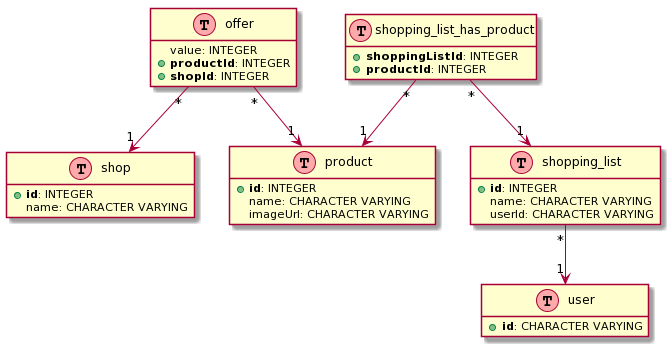
\includegraphics[width=\linewidth]{figuras/MER.png}
\caption{MER da aplicação Price Search.}
\label{fig:mer}
\end{figure}
 
  
 \subsection{Casos de Uso}
O diagrama de casos de uso da aplicação ilustra as ações de um usuário, que tem acesso às funcionalidades listadas, conforme ilustrado na Figura \ref{fig:casos-de-uso}.

\begin{figure}[!htb]
\centering
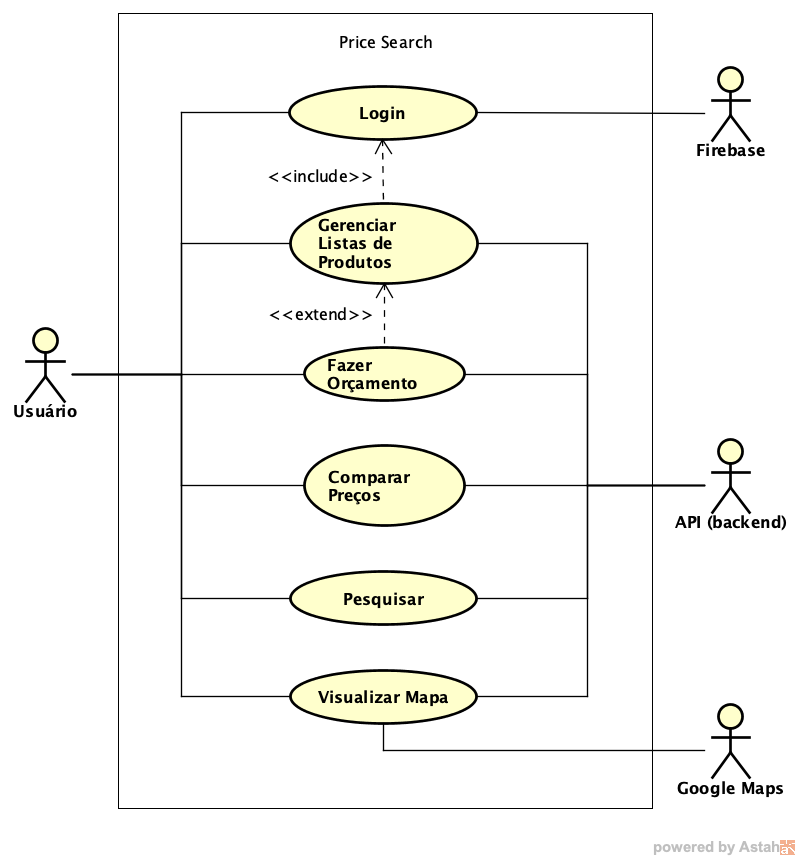
\includegraphics[width=\linewidth]{figuras/DiagramaCasosUsoPriceSearch.png}
\caption{Diagrama de Casos de Uso do Price Search.}
\label{fig:casos-de-uso}
\end{figure}

\subsubsection{Caso de Uso 01: \textit{Login}}

O usuário inicia o \textit{login} (ilustrado na Figura \ref{fig:login}) utilizando uma conta existente do Google, não sendo necessário preenchimento de nenhum tipo de dado pessoal. Feito isto, o assistente valida os dados do usuário e o \textit{login} é efetuado. A aplicação utiliza o ``token'' fornecido pela conta do Google, que é salvo no banco de dados para a sincronização das informações do usuário.

\begin{figure}[H]
\centering
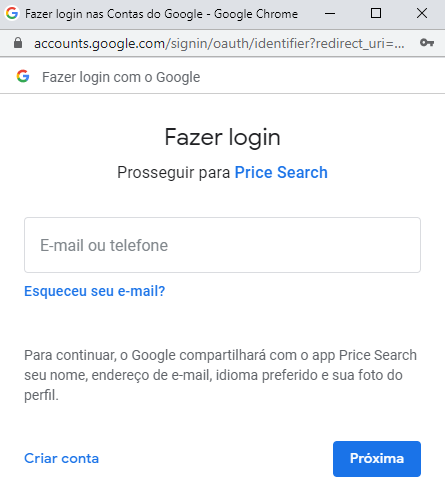
\includegraphics[width=\linewidth]{figuras/tela-login.png}
\caption{Ilustração do Caso de Uso 01: \textit{Login}.}
\label{fig:login}
\end{figure}

\subsubsection{Caso de Uso 02: Pesquisar}

A barra de pesquisa se encontra no topo da página (ilustrado na Figura \ref{fig:menu}); junto dela também existe um botão de menu para mostrar todas as abas do aplicativo. A pesquisa é feita utilizando o nome do produto, então o usuário pode pesquisar por qualquer item, desde que este esteja no banco de dados, e o sistema então retornará todos os itens de acordo com a pesquisa feita realizada.

\begin{figure}[H]
\centering
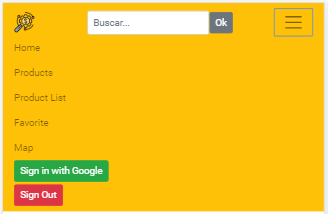
\includegraphics[width=\linewidth]{figuras/tela-menu.png}
\caption{Ilustração do Caso de Uso 02: Pesquisar.}
\label{fig:menu}
\end{figure}

\subsubsection{Caso de Uso 03: Gerenciar Lista de Compra}

O usuário pode criar várias listas de compras, como se fosse um carrinho de compras (ilustrado na Figura \ref{fig:lista}). Ao criar uma lista, o usuário pode escolher um nome para ela, bem como escolher quais itens serão adicionados futuramente e removê-los a qualquer momento, ou mesmo renomear ou excluir a lista.

\begin{figure}[H]
\centering
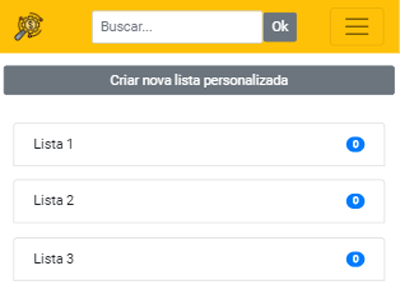
\includegraphics[width=\linewidth]{figuras/tela_lista_personalizada.png}
\caption{Ilustração do Caso de Uso 03: Gerenciar Lista de Compra.}
\label{fig:lista}
\end{figure}

\subsubsection{Caso de Uso 04: Comparar Preços}

O usuário pode comparar preços de um produto em diferentes estabelecimentos (ilustrado na Figura  \ref{fig:comparar}) e, por meio do aplicativo, descobrir em qual estabelecimento ele pode encontrar o melhor preço do produto que deseja.

\begin{figure}[H]
\centering
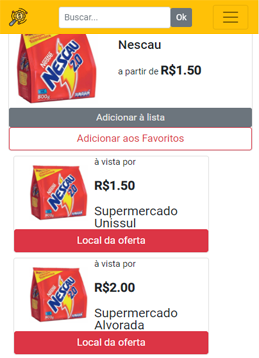
\includegraphics[width=\linewidth]{figuras/tela-comparar.png}
\caption{Ilustração do Caso de Uso 04: Comparar Preços.}
\label{fig:comparar}
\end{figure}

\subsubsection{Caso de Uso 05: Visualizar Mapa}

O usuário tem acesso a um mapa que contém a localização de todos os estabelecimentos locais cadastrados (ilustrado na Figura \ref{fig:mapa}). Ao clicar nos estabelecimentos mostrados no mapa, são fornecidas informações sobre ele, tais como nome e endereço.

\begin{figure}[H]
\centering
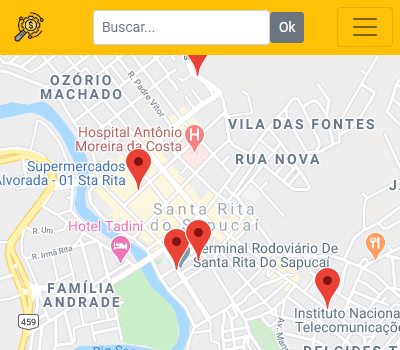
\includegraphics[width=\linewidth]{figuras/tela_mapa.png}
\caption{Ilustração do Caso de Uso 05: Visualizar Mapa.}
\label{fig:mapa}
\end{figure}

\subsection{Integração com os estabelecimentos}

A coleta dos dados é parte fundamental do projeto, e ela pode ser dividida em dois tópicos:
\begin{itemize}
    \item \textbf{A partir de um banco de dados universal}: referido como universal, será dessa fonte que serão coletados os dados estáticos dos produtos, tais como imagens, descrição, identificadores únicos como código de barras, nome, dimensões, peso, entre outros. Essas informações poderão ser coletadas e mantidas regularmente atualizadas por meio do CNP (Cadastro Nacional de Produtos), que é uma API disponibilizada pelo GS1 Brasil\footnote{Disponível em: \url{https://www.gs1br.org/servicos-e-solucoes/cnp-cadastro-nacional-de-produtos}.}.
    \item \textbf{A partir dos bancos de dados dos estabelecimentos}: dados como preços e disponibilidade serão provenientes de cada estabelecimento, e serão interpretados pelos adaptadores responsáveis por realizar a integração nos diferentes estabelecimentos.
\end{itemize}

Uma das principais questões em aberto quanto ao projeto é a respeito de como deverá ser feita a integração com os estabelecimentos locais. Para integrar com o Price Search, esses estabelecimentos precisarão dispor de um sistema de gestão empresarial. Não será possível fazer a integração com estabelecimentos que fazem o controle do estoque manualmente. Dessa forma, é possível abranger um amplo número de locais, ao mesmo tempo em que é mantido os requisitos mínimos necessários para que a integração garanta dados consistentes e atualizados em um tempo razoável.

A integração será desenvolvida respeitando alguns princípios para garantir uma ampla adoção e menor resistência:
\begin{itemize}
    \item \textbf{Transparência}: como as demais partes do projeto, as integrações serão desenvolvidas e disponibilizadas em código aberto. Dessa forma, as empresas podem analisar o código fonte de forma a garantir sua segurança e privacidade. Opcionalmente, a integração poderá prover ao estabelecimento um relatório com o registro das operações realizadas.
    \item \textbf{Baixo compromisso}: os únicos dados que serão requeridos pelo Price Search serão os preços dos produtos (e consequentemente um identificador único de cada produto) e um indicador de disponibilidade do produto, seja em forma de quantidade de itens no estoque, ou como uma variável \textit{booleana} (verdadeiro/falso). Isso garante um compromisso baixo do estabelecimento com a aplicação Price Search, garantindo uma política de privacidade muito pouco invasiva.
    \item \textbf{Baixo custo}: esse tópico pode ser subdividido da seguinte forma:
    \begin{itemize}
        \item \textbf{Custo computacional}: a integração será instalada no ambiente do estabelecimento, de forma a garantir uma conexão segura e estável com o banco de dados do mesmo. Portanto, deve exigir recursos computacionais baixos e preferivelmente suportar eventos, para que a sincronização ocorra sempre que e somente quando for necessário, como no momento em que ocorrer uma alteração de preço.
        \item \textbf{Custo de rede}: não será necessária a sincronização de nenhum dado adicional do produto como imagem e descrição, a não ser seu identificador único. Isso garante um baixo tráfego de dados na rede. Opcionalmente, poderão ser verificado previamente quais produtos tiveram seus preços ou disponibilidade alteradas desde a última sincronização, de forma a não precisar trocar dados redundantes.
        \item \textbf{Custo de implantação}: o sucesso da aplicação depende da quantidade de estabelecimentos sincronizados, e para que seja diminuída a fricção durante sua implantação, a integração não pode gerar custos por parte do Price Search. Será necessário desenvolver documentações completas quanto a essas integrações para que a mesma possa ser implantada de forma simples pelos próprios estabelecimentos ou pelos seus responsáveis de TI (Tecnologia da Informação).
    \end{itemize}
    \item \textbf{Optativo}: de forma simples, os estabelecimentos terão a capacidade de desligar a sincronização ou alterar os dados cadastrais mostrados no Price Search a seu respeito, para que tenham total controle sobre seus dados. 
\end{itemize}

Será necessário o desenvolvimento de adaptadores diferentes para cada sistema de gerenciamento empresarial e/ou banco de dados. Apesar de cada estabelecimento poder utilizar um sistema diferente, o número de diferentes sistemas frente ao de estabelecimentos é muito menor. Com o desenvolvimento de um número limitado de adaptadores será possível suportar uma quantidade grande de estabelecimentos, além de que o desenvolvimento poderá ser feito sob demanda (como quando for encontrado um novo sistema que não for suportado).

\subsection{Testes}

Pretende-se realizar diversos tipos de testes no projeto, tais como:
\begin{itemize}
    \item \textbf{Análise sintática}: capaz de identificar erros de sintaxe do código-fonte, que causariam posteriores erros de compilação. Nesta etapa dos testes também são identificados possíveis más práticas de programação bem como regras de formatação não cumpridas.
    \item \textbf{Teste unitário}: a fim de testar todas as funções de forma isolada, e garantir que uma mudança em uma delas não afete o resultado esperado, que caso contrário, pode causar um mau funcionamento em trechos de código onde essa função é chamada. Também é realizado o teste de cobertura nessa etapa, a fim de saber se todas as funções do código-fonte estão cobertas pelos testes unitários.
    \item \textbf{Testes de integração}: nessa etapa é realizado o teste das APIs REST. Dessa forma, garantimos que os métodos expostos pelo \textit{back-end} e que são utilizados pelo \textit{front-end} continuem a funcionar e a produzir os mesmos resultados esperados, de forma a garantir que uma mudança de código no \textit{back-end} não cause um mau funcionamento no \textit{front-end}.
    \item \textbf{Testes de interface visual}: são responsáveis por simular um usuário real interagindo com a aplicação e por analisar cada um dos casos de usos propostos anteriormente, a fim de garantir seu funcionamento correto.
\end{itemize}

Estes testes, apesar de funcionarem de forma manual, serão executados principalmente de forma automatizada, sempre que e somente quando forem necessários, como por exemplo ao introduzir uma nova mudança no código fonte. Com testes automatizados executando em um ambiente de integração contínua, é possível focar na construção de novas funcionalidades enquanto deixamos os robôs certificarem se o projeto ainda funciona. É uma forma de garantir maior estabilidade ao projeto, necessária principalmente após tê-lo lançado em produção. 
